\documentclass[11pt,a4paper]{article}
\usepackage{gtu-el-yazisi}
\begin{document}
\notbilgi{Elektronik I}{24.05 dersi -- BJT küçük işaret modelleri ve ortak emetörlü yükselteç}{Elektronik-1-24-05.pdf}

\section{Small signal Models}
\noindent\sayfa{1}%
\begin{minipage}[c]{0.45\linewidth}
\centering
\begin{circuitikz}[line width=0.6pt]
  \draw (0,0) node[npn](Q){};
  \draw (Q.B) node[circ]{} node[left]{$B$};
  \draw (Q.C) node[circ]{} node[right]{$C$};
  \draw (Q.E) node[circ]{} node[below]{$E$};
\end{circuitikz}

\medskip
\textcolor{kirmizikalem}{$\pi$ model}

\begin{circuitikz}[line width=0.6pt]
  \draw (0,2) node[circ]{} -- (1,2) to[R, l=$r_\pi$] (1,0) -- (4.4,0);
  \node at (0.6,1.6) {$+$}; \node at (0.4,1) {$V_\pi$}; \node at (0.6,0.4) {$-$};
  \draw (2.8,2) to[cI] (2.8,0);
  \draw (2.8,2) -- (5,2) node[circ]{} node[right]{$C$};
  \draw (4.4,2) to[R, l=$r_o$] (4.4,0);
  \draw (2,0) -- (2,-0.5) node[ocirc]{} node[below]{$E$};
\end{circuitikz}
\[
  v_i\ll V_T\cong 0{,}025\ \text{V}
\]
\end{minipage}\hfill
\begin{minipage}[c]{0.5\linewidth}
\centering
\begin{circuitikz}[line width=0.6pt]
  \draw (0,3.4) to[cI, l=$\alpha i_e$] (0,1.8) to[R, l_=$r_e$, i=$i_e$] (0,0.2) -- (2.4,0.2) to[R, l_=$r_o$] (2.4,3.4) -- (0,3.4);
  \draw (2.4,3.4) -- (3.2,3.4) node[right]{$C$};
  \draw (-1.4,1.8) node[circ]{} node[left]{$B$} -- (0,1.8);
  \draw (1.2,0.2) -- (1.2,-0.4) node[circ]{} node[below]{$E$};
  \node[text=kirmizikalem] at (3.6,2.2) {T model};
\end{circuitikz}
\end{minipage}

\section{Small signal model}
\begin{align*}
  r_o &\rightarrow \text{output resistance of BJT}=\frac{V_A}{I_C} \\
  g_m &\rightarrow \text{transconductance}=\frac{I_C}{V_T} \\
  r_e &\rightarrow \text{emitter resistance}=\frac{V_T}{I_E}\cong 1/g_m \\
  r_\pi &\rightarrow \text{base resistance}=(\beta+1)\cdot r_e
\end{align*}

\section{Practice}
\noindent
\begin{minipage}[c]{0.45\linewidth}
\centering
\begin{circuitikz}[line width=0.6pt]
  \draw (0,0) node[npn](Q){};
  \draw (Q.B) node[left]{$B$};
  \draw (Q.C) node[right]{$C$};
  \draw (Q.E) node[circ]{} node[right]{$E$};
\end{circuitikz}

\medskip
$\pi$ model

\begin{circuitikz}[line width=0.6pt]
  \draw (0,2) node[circ]{} node[left]{$B$} -- (1,2) to[R, l_=$r_\pi$] (1,0) -- (4.4,0);
  \node at (1.4,1.6) {$+$}; \node at (1.6,1.1) {$V_\pi$}; \node at (1.4,0.5) {$-$};
  \draw (2.8,2) to[cI, l=$g_mV_\pi$] (2.8,0);
  \draw (2.8,2) -- (5,2) node[right]{$C$};
  \draw (4.4,2) to[R, l=$r_o$] (4.4,0);
  \draw (2.8,0) -- (2.8,-0.5) node[circ]{} node[below]{$E$};
\end{circuitikz}
\end{minipage}\hfill
\begin{minipage}[c]{0.5\linewidth}
\centering
T model

\begin{circuitikz}[line width=0.6pt]
  \draw (0,3.4) to[cI, l={$\alpha i_e\,/\,g_mV_\pi$}] (0,1.8) to[R, l_=$r_e$, i=$i_e$] (0,0.2) -- (2.8,0.2) to[R, l_=$r_o$] (2.8,3.4) -- (0,3.4);
  \draw (1.4,3.4) -- (1.4,4) node[circ]{} node[right]{$C$};
  \draw (-1.4,1.8) node[ocirc]{} node[left]{$B$} -- (0,1.8);
  \node at (0.9,1.3) {$+$}; \node at (1.2,0.95) {$V_\pi$}; \node at (0.9,0.6) {$-$};
  \draw (0,0.2) node[circ]{} node[below]{$E$};
\end{circuitikz}
\end{minipage}

\noindent\sayfa{2}%
\begin{minipage}[c]{0.58\linewidth}
\centering
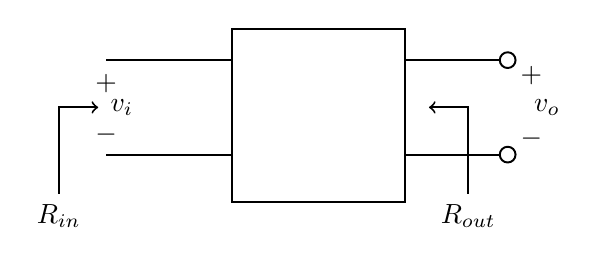
\begin{tikzpicture}[line width=0.7pt]
  \draw (2,0) rectangle (4.2,2.2);
  \draw (0.4,1.8) -- (2,1.8); \draw (0.4,0.6) -- (2,0.6);
  \node at (0.4,1.5) {$+$}; \node at (0.6,1.2) {$v_i$}; \node at (0.4,0.85) {$-$};
  \draw[->] (-0.2,0.1) node[below]{$R_{in}$} -- (-0.2,1.2) -- (0.3,1.2);
  \draw (4.2,1.8) -- (5.4,1.8); \draw (5.5,1.8) circle (0.1);
  \draw (4.2,0.6) -- (5.4,0.6); \draw (5.5,0.6) circle (0.1);
  \node at (5.8,1.6) {$+$}; \node at (6,1.2) {$v_o$}; \node at (5.8,0.8) {$-$};
  \draw[->] (5,0.1) node[below]{$R_{out}$} -- (5,1.2) -- (4.5,1.2);
\end{tikzpicture}
\end{minipage}\hfill
\begin{minipage}[c]{0.38\linewidth}
\underline{Voltage Gain}
\[
  A_v=\frac{v_o}{v_i}
\]
$R_{in}\rightarrow$ Input resistance\\
$R_{out}\rightarrow$ Output
\end{minipage}

\section{Amplifier Topologies}
\begin{itemize}[label=$\llcorner$]
  \item Common Emitter
  \item Common Emitter with $R_E$
  \item Common Base
  \item Common Collector\\ (Emitter-Fol.)
\end{itemize}

\section{Common Emitter amplifier}
\elcizimi[0.9]{sekiller/Elektronik-1-24-05-s2-1.png}[2]

$C_{C1}$, $C_{C2}$, $C_E$ are high values

\medskip
$C$ are open circuit at DC

\noindent
\begin{minipage}[c]{0.55\linewidth}
\centering
\begin{circuitikz}[line width=0.6pt]
  \draw (0,0) node[npn](Q){};
  \draw (Q.C) to[R, l_=$R_C$] ++(0,1.4) node[vcc]{$V_{CC}$};
  \draw (Q.E) to[R, l_=$R_E$] ++(0,-1.4) node[ground]{};
  \draw (Q.B) to[R, l_=$R_{th}$] ++(-1.8,0) coordinate(BB) -- ++(-0.6,0) to[V, invert, l_=$V_{Th}$] ++(0,-1.6) node[ground]{};
\end{circuitikz}
\end{minipage}\hfill
\begin{minipage}[c]{0.4\linewidth}
$g_m$, $r_e$, $r_\pi$, $r_o$
\end{minipage}

\section{@ AC}
\sayfa{3}
\begin{itemize}[label=--]
  \item Now all caps are short circuit
  \item DC voltage sources are short circuit
  \item DC current sources are ``open circuit''
\end{itemize}
\elcizimi[0.8]{sekiller/Elektronik-1-24-05-s3-1.png}[3]

\subsection{Small signal equivalent circuit}
\begin{center}
\begin{circuitikz}[line width=0.6pt]
  \draw (0,0.4) node[ground]{} to[sV, l=$V_{sig}$] (0,2) to[R, l=$R_{sig}$] (1.8,2) -- (3.6,2) node[circ]{} node[above]{$B$};
  \draw (2.0,2) to[R, l={$R_{B1}/\!/R_{B2}$}] (2.0,0.4) node[ground]{};
  \draw[->] (1.2,-0.4) node[below]{$R_{in}$} -- (1.2,1) -- (1.75,1);
  \draw[color=kirmizikalem] (3.6,2) -- (4.4,2) to[R, l=$r_\pi$] (4.4,0.4) -- (7.6,0.4);
  \node[text=kirmizikalem] at (5.3,1.6) {$+$}; \node[text=kirmizikalem] at (5.55,1.2) {$V_\pi$}; \node[text=kirmizikalem] at (5.3,0.7) {$-$};
  \draw[color=kirmizikalem] (6.6,2) to[cI] (6.6,0.4);
  \draw[color=kirmizikalem] (6.6,2) -- (8.4,2);
  \draw[color=kirmizikalem] (7.6,2) to[R, l=$r_o$] (7.6,0.4);
  \draw (8.4,2) node[circ]{} node[above]{$C$} -- (11,2) node[right]{$V_{out}$};
  \draw (9.2,2) to[R, l=$R_C$] (9.2,0.4) node[ground]{};
  \draw (10.6,2) to[R, l=$R_L$] (10.6,0.4) node[ground]{};
  \draw[->] (9.9,-0.4) node[below]{$R_{out}$} -- (9.9,1) -- (9.4,1);
  \node[align=left, font=\small] at (11.9,0.3) {$\downarrow$ Load\\ resistance};
\end{circuitikz}
\end{center}
\elcizimi[0.9]{sekiller/Elektronik-1-24-05-s3-2.png}[3]
\[
  A_v=\frac{v_{out}}{v_{in}},\quad R_{in},\quad R_{out}
\]
\begin{align*}
  R_{in} &= R_{B1}\,/\!/\,R_{B2}\,/\!/\,r_\pi \\
  R_{out} &= R_C\,/\!/\,r_o
\end{align*}

\sayfa{4}
\begin{center}
\begin{circuitikz}[line width=0.6pt]
  \draw (0,0.4) node[ground]{} to[sV, l=$V_{sig}$] (0,2) to[R, l=$R_{sig}$] (1.8,2) -- (3.6,2) node[circ]{} node[above]{$B$};
  \draw (2.0,2) to[R, l={$R_{B1}/\!/R_{B2}$}] (2.0,0.4) node[ground]{};
  \draw[->] (1.2,-0.4) node[below]{$R_{in}$} -- (1.2,1) -- (1.75,1);
  \draw[color=kirmizikalem] (3.6,2) -- (4.4,2) to[R, l=$r_\pi$] (4.4,0.4) -- (7.6,0.4);
  \node[text=kirmizikalem] at (5.3,1.6) {$+$}; \node[text=kirmizikalem] at (5.55,1.2) {$V_\pi$}; \node[text=kirmizikalem] at (5.3,0.7) {$-$};
  \draw[color=kirmizikalem] (6.6,2) to[cI] (6.6,0.4);
  \draw[color=kirmizikalem] (6.6,2) -- (8.4,2);
  \draw[color=kirmizikalem] (7.6,2) to[R, l=$r_o$] (7.6,0.4);
  \draw (8.4,2) node[above]{$C$} -- (10,2) node[right]{$V_{out}$};
  \draw (9.6,2) to[R, l={$R_L'=R_C/\!/r_o/\!/R_L$}] (9.6,0.4) node[ground]{};
\end{circuitikz}
\end{center}
\begin{align*}
  v_{out} &= -g_mV_\pi\cdot R_L' \\
  v_{in} &= v_{sig}
\end{align*}
\[
  v_\pi=\frac{v_{sig}}{R_{sig}+(R_{B1}\,/\!/\,R_{B2}\,/\!/\,r_\pi)}\times(R_{B1}\,/\!/\,R_{B2}\,/\!/\,r_\pi)
\]
\[
  \frac{v_{out}}{v_{sig}}=-\left(\frac{R_{B1}\,/\!/\,R_{B2}\,/\!/\,r_\pi}{\underbrace{R_{sig}+(R_{B1}\,/\!/\,R_{B2}\,/\!/\,r_\pi)}_{\text{Due to large }R_{sig}}}\right)g_m\cdot R_L'
\]
\[
  R_{sig}\approx 0\ \Rightarrow\ =-g_m\,R_L'
\]
\begin{itemize}[label=$\rightarrow$]
  \item High Voltage Gain $\cong -g_mR_L'$
  \item Moderate Input Resistance $\rightarrow R_{B1}\,/\!/\,R_{B2}\,/\!/\,r_\pi$
  \item '' High output Resistance $\rightarrow R_C\,/\!/\,r_o$
\end{itemize}

\hfill $R_{in}$ büyük olsun isteriz

\noindent
\begin{minipage}[c]{0.45\linewidth}
\centering
\begin{circuitikz}[line width=0.6pt]
  \draw (0,1.6) to[R, l=$R_{out}$] (2,1.6) -- (3,1.6) node[right]{$V_{out}$};
  \draw (2,1.6) to[R, l=$R_L$] (2,0) node[ground]{};
\end{circuitikz}
\end{minipage}\hfill
\begin{minipage}[c]{0.5\linewidth}
$R_{out}$ küçük olmasını isteriz
\end{minipage}

\section{Common Emitter amplifier with $R_E$}
\noindent\sayfa{5}
\elcizimi[0.8]{sekiller/Elektronik-1-24-05-s5-1.png}[5]

\noindent \underline{Use t model} \hfill $R_B=R_{B1}\,/\!/\,R_{B2}$
\begin{center}
\begin{circuitikz}[line width=0.6pt]
  \draw (0,0.4) node[ground]{} to[sV, l=$V_{sig}$] (0,2) to[R, l=$R_{sig}$] (1.8,2) -- (3.6,2) node[circ]{} node[above]{$B$};
  \draw (2.0,2) to[R, l={$R_{B1}/\!/R_{B2}$}] (2.0,0.4) node[ground]{};
  \draw[->] (1.2,-0.4) node[below]{$R_{in}$} -- (1.2,1) -- (1.75,1);
  \draw[<-] (3.75,2.1) -- (4.2,2.6) node[right]{$v_B$};
  \draw[color=kirmizikalem] (3.6,2) -- (4.4,2) to[R, l=$r_\pi$] (4.4,0.4) -- (7.6,0.4);
  \node[text=kirmizikalem] at (5.3,1.6) {$+$}; \node[text=kirmizikalem] at (5.55,1.2) {$V_\pi$}; \node[text=kirmizikalem] at (5.3,0.7) {$-$};
  \draw[color=kirmizikalem] (6.6,2) to[cI] (6.6,0.4);
  \draw[color=kirmizikalem] (6.6,2) -- (8.4,2);
  \draw[color=kirmizikalem] (7.6,2) to[R, l=$r_o$] (7.6,0.4);
  \draw (8.4,2) node[circ]{} node[above]{$C$} -- (11,2) node[right]{$V_{out}$};
  \draw (9.2,2) to[R, l=$R_C$] (9.2,0.4) node[ground]{};
  \draw (10.6,2) to[R, l=$R_L$] (10.6,0.4) node[ground]{};
  \draw[->] (9.9,-0.4) node[below]{$R_{out}$} -- (9.9,1) -- (9.4,1);
  \draw[color=kirmizikalem] (5.4,0.4) -- (5.4,-0.2) node[ocirc]{} node[right]{$E$};
  \draw (5.4,-0.2) to[R, l=$R_E$] (5.4,-1.8) node[ground]{};
  \node at (4.8,-0.4) {$+$}; \node at (4.5,-1) {$v_x$}; \node at (4.8,-1.5) {$-$};
\end{circuitikz}
\end{center}
$V_A=\infty$, $r_o=\infty$
\begin{align*}
  R_{in} &= R_B\,\bigl(r_\pi+R_E(\beta+1)\bigr) \\
  &= R_B\,/\!/\,\bigl[(\beta+1)\,(r_e+R_E)\bigr] \\
  R_{out} &\cong R_C \\
  A_v &= \frac{v_{out}}{v_{in}}
\end{align*}
\[
  v_{out}=-g_mV_\pi\,(R_C\,/\!/\,R_L) \qquad\qquad V_\pi\overset{?}{=}V_{sig}
\]
\begin{align*}
  v_x &= \left(g_mV_\pi+\frac{V_\pi}{r_\pi}\right)R_E \\
  &= \left(\frac{V_\pi}{r_e}+\frac{V_\pi}{r_\pi}\right)R_E\cong\frac{v_\pi}{r_e}\cdot R_E \\
  v_b &= v_\pi\left(1+\frac{R_E}{r_e}\right)
\end{align*}
if $R_{sig}\approx 0$ \quad $v_b=v_{sig}$

\sayfa{6}
\[
  \frac{v_{out}}{v_{in}}=\frac{-g_m\,\rlap{$\diagup$}V_\pi\,(R_C\,/\!/\,R_L)}{\rlap{$\diagup$}V_\pi\left(1+\frac{R_E}{r_e}\right)} \qquad\qquad r_e=\frac{1}{g_m}
\]
\[
  \frac{v_{out}}{v_{in}}=\frac{-g_m\,(R_C\,/\!/\,R_L)}{r_e\left(1+\frac{R_E}{r_e}\right)}\ \text{\footnotemark}
  \ \cong-\frac{(R_C\,/\!/\,R_L)}{r_e+R_E}
\]
\footnotetext{Claude notu: $g_m=1/r_e$ yerine konduğunda payda $g_m$ kalmamalı, yani $-\dfrac{(R_C/\!/R_L)}{r_e(1+R_E/r_e)}$ olmalı; son sonuç doğru.}
\[
  A_v\cong-\frac{R_C\,/\!/\,R_L}{R_E+r_e}
\]

\noindent
\begin{minipage}[c]{0.5\linewidth}
\centering
\begin{circuitikz}[line width=0.6pt]
  \draw (0,0) node[ground]{} to[sV, l=$V_{sig}$] (0,1.6) to[R, l=$R_{sig}$] (2,1.6) -- (3.4,1.6) node[circ]{};
  \draw (2.2,1.6) to[R, l_=$R_B$] (2.2,0) node[ground]{};
  \draw (3.4,3.4) to[cI, l=$\beta i_e$] (3.4,1.6) to[R, l=$r_e$] (3.4,0.1) to[R, l=$R_E$] (3.4,-1.4) node[ground]{};
  \node at (4.4,0.85) {$\downarrow i_e$};
  \draw[->] (3.4,1.6) -- (4.3,1.6) node[right]{$V_x$};
  \draw (3.4,3.4) -- (6.2,3.4) node[right]{$V_{out}$};
  \draw (5.2,3.4) to[R, l={$R_C/\!/R_L$}] (5.2,1.8) node[ground]{};
\end{circuitikz}
\end{minipage}\hfill
\begin{minipage}[c]{0.45\linewidth}
\centering
\tikz[baseline=(c.base)]\node[draw,circle,inner sep=1pt](c){\small 2};\\
$\Big\}\rightarrow$ \fbox{$v_x=i_e\,(R_E+r_e)$}\\
\textcolor{kirmizikalem}{\okunamadi{$V_{sig}\neq i_e\,(R_E+r_e)$}}

\bigskip
\tikz[baseline=(c.base)]\node[draw,circle,inner sep=1pt](c){\small 3};
\[
  \frac{v_{out}}{\textcolor{kirmizikalem}{V_{sig}}}=\frac{-\alpha\,i_e\,(R_C\,/\!/\,R_L)}{\textcolor{kirmizikalem}{i_e\,(R_E+r_e)}}
\]
\end{minipage}

\begin{center}
\begin{circuitikz}[line width=0.6pt]
  \draw (0,0) node[ground]{} to[sV, l=$V_{sig}$] (0,1.6) to[R, l=$R_{sig}$] (2,1.6) -- (4,1.6) node[above]{$V_x$};
  \draw (2.4,1.6) to[R, l=$R_B$] (2.4,0);
  \draw (4,1.6) to[R, l={$(\beta+1)(r_e+R_E)$}] (4,0) node[ground]{};
\end{circuitikz}
\end{center}
\[
  V_x=\frac{(\beta+1)(r_e+R_E)\,/\!/\,R_B\cdot V_{sig}}{R_{sig}+\underbrace{(\beta+1)(r_e+R_E)\,/\!/\,R_B}_{\textcolor{kirmizikalem}{\downarrow\ T}}}
\]
\begin{center}
\textcolor{kirmizikalem}{$R_{signal}\ll T$}
\end{center}

\sayfa{7}
\noindent Validation

\noindent
\begin{minipage}[c]{0.45\linewidth}
\centering
\begin{circuitikz}[line width=0.6pt]
  \draw (0,0) node[npn](Q){};
  \draw (Q.C) to[R, l_=$R_C$] ++(0,1.6) node[vcc]{};
  \draw[->] (Q.C) -- ++(1,0) node[right]{$V_{out}$};
  \draw (Q.E) to[R, l_=$R_E$] ++(0,-1.6) node[ground]{};
  \draw (Q.B) -- ++(-1,0) to[sV, l_=$V_{sig}$] ++(0,-1.4) node[ground]{};
\end{circuitikz}
\end{minipage}\hfill
\begin{minipage}[c]{0.5\linewidth}
\[
  \textcolor{kirmizikalem}{A_v=-\frac{R_C}{R_E}}
\]
\begin{itemize}[label={}, leftmargin=1em]
  \item High input Imp
  \item Low voltage gain
  \item More output Imp
  \item More stable
  \item Independent of $g_m$
  \item High bandwidth
\end{itemize}
\end{minipage}

\end{document}
